% !TEX program = xelatex
\documentclass[zihao=-4,a4paper]{ctexart}
\usepackage{fontspec}
\usepackage{xeCJK}
\usepackage{amsmath,amssymb,bm}
\usepackage{graphicx}
\usepackage{listings}
\usepackage{xcolor}
\usepackage{float}
\usepackage{enumitem}
\usepackage{caption}
\usepackage{booktabs}
\usepackage{array}
\usepackage{changepage} % 用于调整局部正文的左右边距
\usepackage{pdfpages}
\setmonofont{Consolas}   % 设置等宽字体为 Consolas
\setCJKmainfont{SimSun}[AutoFakeBold=2.5]
\usepackage{hyperref}
% 页面布局
\usepackage[
  top    = 1.7cm,
  left   = 1.7cm,
  right  = 1.7cm,
  bottom = 2.7cm,
  footskip = 1cm
]{geometry}
\linespread{1.5}
% 提供 current page text area 节点
\usepackage{tikzpagenodes}
\usetikzlibrary{calc}            % 用于计算坐标
\usepackage{fancyhdr}
% ==============================
% 全局变量: 存储版心宽度
% ==============================
\newlength{\myTextWidth}
\newcommand{\calcTextWidth}{%
  \path let \p1=(current page text area.east), \p2=(current page text area.west) in 
    \pgfextra{\pgfmathsetlength{\myTextWidth}{\x1-\x2}};
}

% ==============================
% 背景画线逻辑
% ==============================
\newif\ifdrawbackground  % 定义背景绘制开关
\drawbackgroundtrue      % 默认开启背景绘制
\AddToHook{shipout/background}{%
  \ifdrawbackground %只有开关开启时才绘制背景
  \tikz[remember picture, overlay]{%
    
    % 定义上下外扩的距离(和表格撑开的距离保持一致)
    \def\vpad{0.8em} 

    % --- 所有页: 底部横线 (向下偏移 \vpad) ---
    \draw[line width=1pt] 
      ([yshift=-\vpad]current page text area.south west) -- 
      ([yshift=-\vpad]current page text area.south east);

    \ifnum\value{page}=1
      % --- 第一页: 绘制 2x6 表格边框 ---
      \def\innerLineWidth{0.8pt}
      \def\outerLineWidth{1pt}

      % 1. 上横线 (表格节点已通过 inner ysep 撑开, 直接画)
      \draw[line width=\outerLineWidth] 
        (title-bottom-mark -| current page text area.west) -- 
        (title-bottom-mark -| current page text area.east);

      % 2. 下横线 (同上)
      \draw[line width=\outerLineWidth] 
        (table-bottom-mark -| current page text area.west) -- 
        (table-bottom-mark -| current page text area.east);

      % 3. 中间横线 (自动居中)
      \draw[line width=\innerLineWidth] 
        ($(title-bottom-mark -| current page text area.west)!0.5!(table-bottom-mark -| current page text area.west)$) -- 
        ($(title-bottom-mark -| current page text area.east)!0.5!(table-bottom-mark -| current page text area.east)$);

      % 4. 左右外框竖线 (从表格顶部一直到页底, 页底向下偏移 \vpad)
      \draw[line width=\outerLineWidth] 
        (title-bottom-mark -| current page text area.west) -- 
        ([yshift=-\vpad]current page text area.south west);
      \draw[line width=\outerLineWidth] 
        (title-bottom-mark -| current page text area.east) -- 
        ([yshift=-\vpad]current page text area.south east);

      % 5. 内部竖线 (5条)
      \foreach \i in {1,2,...,5} {
        \pgfmathsetmacro{\pos}{\i/6}
        \draw[line width=\innerLineWidth]
          ($(title-bottom-mark -| current page text area.west)! \pos !(title-bottom-mark -| current page text area.east)$) --
          ($(table-bottom-mark -| current page text area.west)! \pos !(table-bottom-mark -| current page text area.east)$);
      }

    \else
      % --- 后续页: 标准四周边框 (上下各外扩 \vpad) ---
      % 顶部横线向上偏移
      \draw[line width=1pt] ([yshift=\vpad]current page text area.north west) -- ([yshift=\vpad]current page text area.north east);
      % 左右竖线跟随上下偏移
      \draw[line width=1pt] ([yshift=\vpad]current page text area.north west) -- ([yshift=-\vpad]current page text area.south west);
      \draw[line width=1pt] ([yshift=\vpad]current page text area.north east) -- ([yshift=-\vpad]current page text area.south east);
    \fi
  }%
  \fi
}


\pagestyle{fancy}
\fancyhf{}
\fancyfoot[C]{\thepage}
\renewcommand{\headrulewidth}{0pt}

% 直接使用 \textwidth 计算列宽
% ==============================
% \textwidth/6 保证精确6等分, 减去 2\tabcolsep 扣除单元格自带的左右边距
\newcolumntype{C}{>{\raggedright\arraybackslash}p{\dimexpr\textwidth/6-2\tabcolsep\relax}}

% 自定义命令: 在当前位置画一条贯穿全宽的横线
% ==============================
\newcommand{\addhline}{%
  \par
  \noindent
  \begin{tikzpicture}[remember picture, overlay]
    % (0,0) 代表当前文字所在的高度
    % current page text area.west 代表版心最左侧
    % |- 符号表示: 取左边的 X 坐标, 取右边的 Y 坐标
    \draw[line width=1pt] 
      (current page text area.west |- 0,0) -- 
      (current page text area.east |- 0,0);
  \end{tikzpicture}\par
}

\newcommand{\dd}{\mathop{}\!\mathrm{d}}

\begin{document}

% 插入封面：临时关闭背景绘制 + 清空页眉页脚 + 不占页码
\drawbackgroundfalse
\pagestyle{empty}
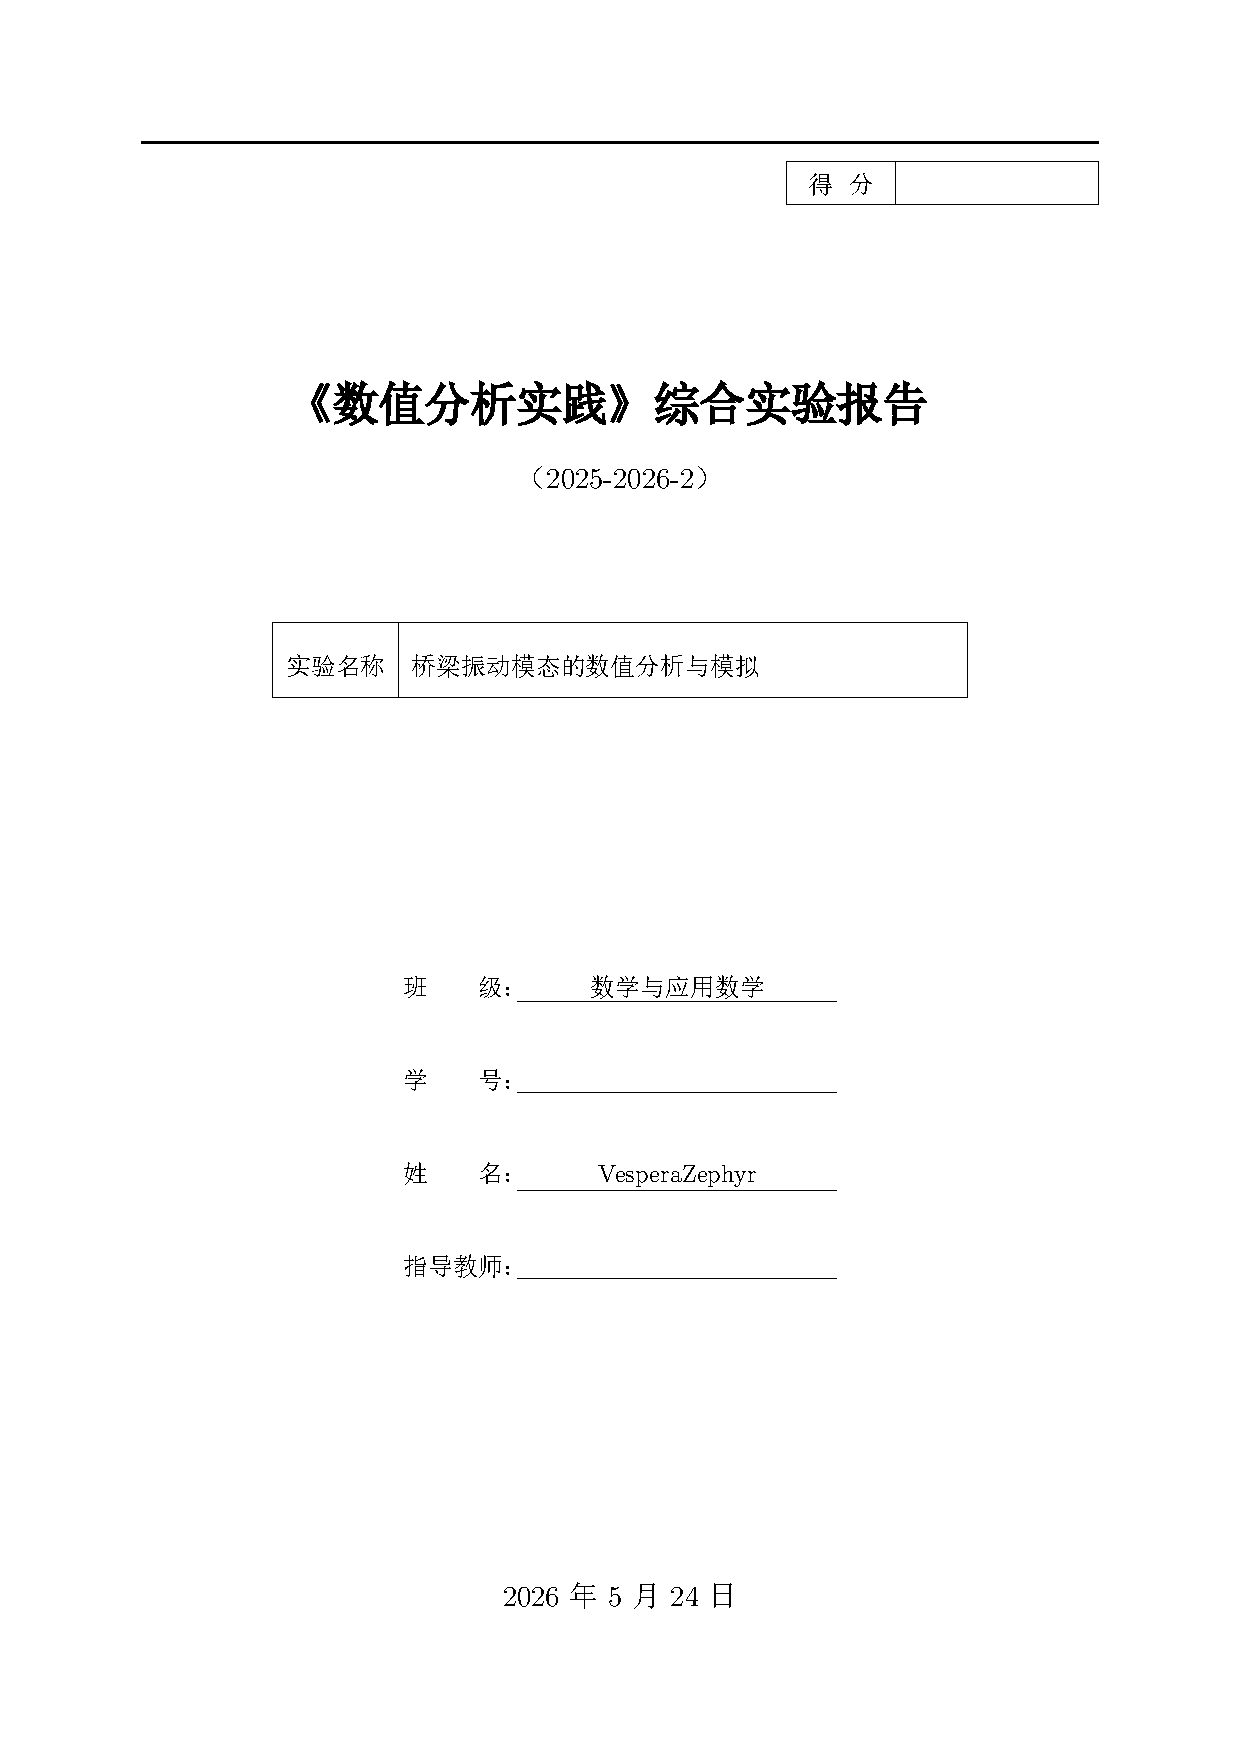
\includepdf[pages={1}]{封面.pdf}
\drawbackgroundtrue  % 恢复背景绘制
\pagestyle{fancy}    % 恢复你的页眉页脚
\setcounter{page}{1} % 重置页码，正文从第1页开始（完美兼容你原来的 \ifnum\value{page}=1 逻辑）

\begin{center}
  \zihao{-2}\bfseries 《数值分析实践》综合实验报告
\end{center}

% --- 表格内容区 ---
\noindent
\begin{tikzpicture}[remember picture]
  % 将整个 tabular 放入一个 TikZ 节点中, 彻底屏蔽 LaTeX 段落间距的干扰
  \node[anchor=north west, inner sep=0pt, outer sep=0pt] (header-table) at (0,0) {%
    \renewcommand{\arraystretch}{1.8}% 增加行高
    \begin{tabular}{CCCCCC} 
      姓\quad 名 &  & 班\quad 级 & \small  & 报告评分 & \\
      学\quad 号 &  & 地点/机号 &  & 指导教师 & 
    \end{tabular}%
  };
  
  % 自动获取这个表格真实的左上角和左下角坐标, 传给背景画线
  \coordinate (title-bottom-mark) at (header-table.north west);
  \coordinate (table-bottom-mark) at (header-table.south west);
\end{tikzpicture}

\setlength{\leftskip}{1em}
\setlength{\rightskip}{1em}

% 实验名称
\noindent{\bfseries 一、实验名称: 桥梁振动模态的数值分析与模拟}

\addhline

% --- 正文开始 ---
\noindent\textbf{【背景简介】} 在桥梁健康监测中, 振动模态分析是关键手段. 通过传感器测量桥梁某截面在多个频率激励下的位移响应, 可建立线性系统模型. 已知桥梁结构可简化为一个二阶微分方程, 其离散化后得到线性代数系统, 需综合运用多种数值方法进行分析. 

\noindent\textbf{【实验内容】} 考虑如下两点边值问题, 描述桥梁在单位荷载下的静态变形 $u(x)$: 
\[
\begin{cases}
\displaystyle -\frac{\dd^2u}{\dd x^2} + c(x)u = f(x),& x\in[0,L];\\[4pt]
u(0)=0,\quad u(L)=0.
\end{cases}
\]
其中 $L=10,\ c(x)=1+0.5\sin(x),\ f(x)=\sin(\pi x/L)$. 

离散化后的线性系统: 将区间$[0,L]$等分为$n$个子区间($n=20,40,80$), 步长$h=L/n$, 节点 $x_i=ih\ (i=0,1,\cdots,n)$. 采用中心差分
\[
u''(x_i)\approx \frac{\dd^2u}{\dd x^2}\bigg|_{x_i} \approx \frac{u_{i+1}-2u_i+u_{i-1}}{h^2}
\]
离散后(离散截断误差为 $O(h^2)$, 具备二阶精度)得到三对角线性方程组 $\bm{Au}=\bm{b}$, 其中
\begin{enumerate}[label=(\arabic*)]
\item $\bm{u}=(u_1,u_2,\cdots,u_{n-1})^\top,\ u_i\approx u(x_i)$
\item 矩阵$\bm{A}$为三对角对称正定矩阵: 
\[
\bm{A}=\frac1{h^2}\mathrm{tridiag}(-1,2,-1)+\mathrm{diag}\big(c(x_1),c(x_2),\cdots,c(x_{n-1})\big)
\]
\item 右端项
\[
b_i=f(x_i),\ i=1,2,\cdots,n-1
\]
\end{enumerate}

\noindent\textbf{要求: }自行构造出$\bm{A}$和$\bm{b}$的显式形式(用代码生成). 

\addhline

\noindent\textbf{【实验步骤】}

\noindent\textbf{1. 线性方程组求解: } (1) 使用 LU 分解(不选主元)求解 $n=20,40,80$ 时的数值解; 任意选择一种迭代方法求解同一问题(验证$A$对称正定); 并将两个方法的数值解画在一个图上展示; (2) 对两种方法的计算时间进行比较(使用 \texttt{tic/toc} 或 \texttt{time.time()} 等工具). 

\noindent\textbf{2. 误差分析: } 取 $n=160$ 的解为``精确参考解''(用 LU 分解得到), 计算不同 $n$ 下的相对误差: 
\[
E_{\rm rel}=\frac{\|\bm{u}_n-\bm{u}_{\rm ref}\|_2}{\|\bm{u}_{\rm ref}\|_2},
\]
通过画图分析误差随 $h$ 的变化趋势, 验证收敛阶. 

\noindent\textbf{3. 插值与数值积分: } 
(1)从 $n=20$ 的数值解中, 选取 $m=5$ 个等距节点(不含端点), 构造三次样条插值函数 $S(x)$; 
(2)用 $S(x)$ 计算 $x=3.75$ 处的位移值, 并与参考解比较; 
(3)使用复合辛普森法则(步长 $h_{\rm int}=0.1$)计算桥梁中点附近的平均变形: 
\[
I=\frac12\int_{4}^{6}u(x)\dd x.
\]
用参考解近似真值(你不需要知道 $u(x)$ 的解析形式, 用原始数值解构造三次样条, 再对样条求值, 就能得到 $u(x_{\rm int})$). 

\noindent\textbf{4. 扰动敏感性分析: }  在 $n=40$ 时, 对右端项 $\bm b$ 添加随机相对扰动 $\delta=10^{-6}$(即 $\tilde b_i = b_i(1+\varepsilon_i),\ \varepsilon_i\sim \mathcal{N}(0,\delta^2)$), 重新求解方程组, 计算: 
\[
\frac{\|\tilde{\bm u}-\bm u\|_2}{\|\bm u\|_2}\quad \text{与}\quad \frac{\|\tilde{\bm b}-\bm b\|_2}{\|\bm b\|_2}
\]
解释结果与矩阵条件数的关系. 

\addhline
\noindent\textbf{三、问题求解}

对内点 $x_i\;(i=1,2,\cdots,n-1)$, 有  
\[
-\frac{u_{i-1}-2u_i+u_{i+1}}{h^2} + c(x_i)u_i = f(x_i).
\]  
整理得  
\[
-\frac{1}{h^2}u_{i-1} + \left(\frac{2}{h^2}+c(x_i)\right)u_i - \frac{1}{h^2}u_{i+1} = f(x_i),
\qquad i=1,\cdots,n-1,
\]  
边界条件 $u_0=u_n=0$. 

令 $\bm{u}:=[u_1,u_2,\cdots,u_{n-1}]^\top$, 则系统为  
\[
\bm{Au} = \bm{b},
\]  
其中  
\[
\bm{A} = \frac{1}{h^2}
\begin{pmatrix}
2+h^2c_1 & -1 & & & 0 \\
-1 & 2+h^2c_2 & -1 & \\
& \ddots & \ddots & \ddots \\
& & -1 & 2+h^2c_{n-2} & -1 \\
0 & & & -1 & 2+h^2c_{n-1}
\end{pmatrix},\quad
\bm{b} = \begin{pmatrix} f(x_1) \\ f(x_2) \\ \vdots \\ f(x_{n-1}) \end{pmatrix}.
\]
矩阵 $\bm{A}$ 为对称三对角阵, 且严格对角占优(每行对角元 $>$ 同行非对角元模之和), 故对称正定. 

\noindent\textbf{3.1 线性方程组求解}

\noindent\textbf{3.1.1 不选主元的LU分解法}

三对角矩阵 $\bm{A}$ 可作不选主元的 LU 分解 $\bm{A} = \bm{LU}$, 其中  
\[
\bm{L} = \begin{pmatrix}
1 & 0 & & \\
\ell_2 & 1 & \ddots & \\
& \ddots & \ddots & 0 \\
& & \ell_{n-1} & 1
\end{pmatrix},\quad
\bm{U} = \begin{pmatrix}
\alpha_1 & \beta_1 & & \\
0 & \alpha_2 & \beta_2 & \\
& \ddots & \ddots & \beta_{n-2} \\
& & 0 & \alpha_{n-1}
\end{pmatrix}.
\]
\noindent \textbf{算法步骤: }
\begin{enumerate}
    \item \textbf{初始化}:  
    \[
    \alpha_1 = d_1,\qquad \beta_1 = -\frac{1}{h^2},
    \]  
    这里记 $d_i = \frac{2}{h^2}+c(x_i)$, 非对角线元素 $a_i = -\frac{1}{h^2}$(所有 $a_i$ 相同). 

    \item \textbf{分解递推}($i=2,3,\cdots,n-1$):  
    \[
    \ell_i = \frac{a_{i-1}}{\alpha_{i-1}} = \frac{-1/h^2}{\alpha_{i-1}},
    \qquad
    \alpha_i = d_i - \ell_i \beta_{i-1} = d_i - \ell_i\left(-\frac{1}{h^2}\right).
    \]  
    若 $i<n-1$, 则 $\beta_i = -\frac{1}{h^2}$, 否则无 $\beta_i$. 

    \item \textbf{前向代入(求 $\bm{Ly}=\bm{b}$)}:
    \[
    y_1 = b_1,
    \qquad
    y_i = b_i - \ell_i\, y_{i-1},\quad i=2,\cdots,n-1.
    \]

    \item \textbf{回代(求 $\bm{Uu}=\bm{y}$)}:  
    \[
    u_{n-1} = \frac{y_{n-1}}{\alpha_{n-1}},
    \qquad
    u_i = \frac{y_i - \beta_i u_{i+1}}{\alpha_i},\quad i=n-2,\cdots,1.
    \]
\end{enumerate}
由于 $\bm{A}$ 严格对角占优, 上述分解不会出现零主元, 无需选主元, 数值稳定. 

\vspace*{1em}
\noindent\textbf{3.1.2 迭代解法: Gauss-Seidel迭代法}

将系数矩阵 $\bm{A}$ 分解为
\[
\bm{A} = \bm{D} - \bm{L} - \bm{U},
\]
其中 $\bm{D}$ 是对角矩阵(主对角线元素), $-\bm{L}$ 是严格下三角部分, $-\bm{U}$ 是严格上三角部分. 对于本问题的三对角矩阵, 有: 
\begin{itemize}
    \item $\bm{D} = \operatorname{diag}(d_1, d_2, \cdots, d_{n-1})$, 其中 $d_i = \frac{2}{h^2}+c_i$. 
    \item $\bm{L}$ 的下三角非零元为 $-\frac{1}{h^2}$(在次对角线上). 
    \item $\bm{U}$ 的上三角非零元为 $-\frac{1}{h^2}$(在次对角线上). 
\end{itemize}

Gauss-Seidel 迭代公式为: \textbf{向量形式}为
\[
(\bm{D} - \bm{L})\bm{u}^{(k+1)} = \bm{U}\bm{u}^{(k)} + \bm{b}.
\]
或等价地,
\[
\bm{u}^{(k+1)} = (\bm{D} - \bm{L})^{-1}\left(\bm{U}\bm{u}^{(k)} + \bm{b}\right).
\]

对于本问题的三对角结构, 每个分量的更新公式为: 
\begin{enumerate}
    \item \textbf{初始化}: 选取初始向量 $\bm{u}^{(0)}$(通常取零向量), 给定收敛容差 $\varepsilon$ 和最大迭代次数 $K_{\max}$. 
    \item \textbf{迭代}: 对 $k=0,1,2,\cdots$ 直到收敛: 
    \begin{itemize}
        \item 对 $i = 1$(第一个方程, 注意 $u_0=0$): 
        \[
        u_1^{(k+1)} = \frac{1}{d_1}\left(b_1 + \frac{1}{h^2}u_2^{(k)}\right).
        \]
        \item 对 $i = 2,3,\cdots, n-2$(中间方程): 
        \[
        u_i^{(k+1)} = \frac{1}{d_i}\left(b_i + \frac{1}{h^2}u_{i-1}^{(k+1)} + \frac{1}{h^2}u_{i+1}^{(k)}\right).
        \]
        \item 对 $i = n-1$(最后一个方程, 注意 $u_n=0$): 
        \[
        u_{n-1}^{(k+1)} = \frac{1}{d_{n-1}}\left(b_{n-1} + \frac{1}{h^2}u_{n-2}^{(k+1)}\right).
        \]
        \item 计算相邻迭代的差值: 
        \[
        \delta^{(k+1)} = \max_{1\leq i\leq n-1} |u_i^{(k+1)} - u_i^{(k)}|.
        \]
        \item 若 $\delta^{(k+1)} < \varepsilon$, 则迭代收敛, 退出; 若达到最大迭代次数, 则输出警告后终止. 
    \end{itemize}
\end{enumerate}

在更新 $u_i$ 时, 已使用同一次迭代中刚算出的 $u_{i-1}^{(k+1)}$, 以及上一轮迭代的 $u_{i+1}^{(k)}$, 体现了“即时更新”的特点. 

对于本问题, 非对角元均为 $-\frac{1}{h^2}$, 因此公式中的 $\bm{L}$ 和 $\bm{U}$ 的符号已隐含(即原方程左端为 $-a_{i,i-1}u_{i-1} + d_i u_i - a_{i,i+1}u_{i+1} = b_i$, 移项后得到上述显式公式). 由于 $\bm{A}$ 严格对角占优且对称正定, Gauss-Seidel 迭代对任意初始向量均收敛. 收敛速度由矩阵的谱半径决定: 
\[
\rho\left((\bm{D}-\bm{L})^{-1}\bm{U}\right) < 1.
\]
实际实现中, 使用相邻两次解的最大差小于给定容差(如 $\varepsilon = 10^{-8}$)作为停机标准, 同时设置最大迭代次数防止死循环. 

\noindent\textbf{3.2 误差分析}

采用\textbf{有限差分算法}. 算法步骤如下:

\begin{enumerate}[label=\textbf{\arabic*.}, leftmargin=1cm, rightmargin=0.5cm]

    \item \textbf{问题设置与参数初始化}
    \begin{itemize}
        \item 设定区间长度 $L = 10$, 定义系数函数 $c(x)$ 和右端函数 $f(x)$. 
        \item 指定待测试的网格划分数列表 $n_{\text{list}} = [20, 40, 80]$(内点数 $N = n-1$). 
        \item 边界条件为齐次 Dirichlet 条件. 
    \end{itemize}

    \item \textbf{生成参考解(极细网格)}
    \begin{enumerate}[label=(\arabic*)]
        \item 取参考网格划分数 $n_{\text{ref}} = 1280$, 计算步长 $h_{\text{ref}} = L/n_{\text{ref}}$. 
        \item 生成均匀网格节点 $x_{\text{ref}} = \text{linspace}(0, L, n_{\text{ref}}+1)$, 提取内部节点
        $x_{\text{ref,in}} = x_{\text{ref}}(2:n_{\text{ref}})$, 内点个数 $N_{\text{ref}} = n_{\text{ref}}-1$. 
        \item 构造三对角系数矩阵 $\bm{A}_{\text{ref}} \in \mathbb{R}^{N_{\text{ref}} \times N_{\text{ref}}}$: 
        \begin{itemize}
            \item 主对角线: $\displaystyle \frac{2}{h_{\text{ref}}^2} + c(x_{\text{ref,in}})$, 
            \item 上、下次对角线: $\displaystyle -\frac{1}{h_{\text{ref}}^2}$. 
        \end{itemize}
        该矩阵来源于中心差分离散: 
        \[
        -\frac{u_{i-1} - 2u_i + u_{i+1}}{h^2} + c_i u_i = f_i.
        \]
        \item 构造右端向量 $\bm{b}_{\text{ref}} = f(x_{\text{ref,in}})$. 
        \item 求解线性方程组 $\bm{A}_{\text{ref}} \bm{u}_{\text{ref}} = \bm{b}_{\text{ref}}$, 获得参考解向量 $\bm{u}_{\text{ref}}$. 
    \end{enumerate}

    \item \textbf{对不同粗网格求解并计算误差}
    
    对每个 $k$(对应 $n = 20, 40, 80$)依次执行以下步骤: 
    \begin{enumerate}[label=(\arabic*)]
        \item 计算当前步长 $h = L/n$, 并记录 $h_{\text{vals}}(k) = h$. 
        \item 生成网格节点 $x = \text{linspace}(0, L, n+1)$, 取内部节点 $x_{\text{in}} = x(2:n)$, 内点数 $N = n-1$. 
        \item 按照与参考解相同的差分格式, 构造当前粗网格的系数矩阵 $\bm{A} \in \mathbb{R}^{N \times N}$ 和右端向量 $\bm{b} = f(x_{\text{in}})$. 
        \item 求解线性方程组 $\bm{A} \bm{u}_n = \bm{b}$, 得到数值解 $\bm{u}_n$. 
        \item 从参考解中提取对应粗网格内点的值: 
        利用网格点数比例 $r = n_{\text{ref}}/n$(整数), 索引为 $\text{idx}_{\text{ref}} = (1:N)^{\top} \cdot r$, 则
        \[
        \bm{u}_{\text{ref,coarse}} = \bm{u}_{\text{ref}}(\text{idx}_{\text{ref}}).
        \]
        \item 计算相对误差($2$‑范数)并存储: 
        \[
        E_{\text{rel}}(k) = \frac{\| \bm{u}_n - \bm{u}_{\text{ref,coarse}} \|_2}{\| \bm{u}_{\text{ref,coarse}} \|_2}.
        \]
        \item 输出当前网格的 $n$、$h$ 和 $E_{\text{rel}}$. 
    \end{enumerate}

    \item \textbf{收敛阶估计}
    \begin{itemize}
        \item 若网格数不少于 $3$, 利用相邻误差比估计收敛阶: 
        \[
        p_1 = \log_2 \left( \frac{E_{\text{rel}}(n=20)}{E_{\text{rel}}(n=40)} \right), \quad
        p_2 = \log_2 \left( \frac{E_{\text{rel}}(n=40)}{E_{\text{rel}}(n=80)} \right).
        \]
        \item 显示估计值 $p_1$、$p_2$, 预期均接近 $2$(二阶收敛). 
    \end{itemize}
  \end{enumerate}

\noindent\textbf{3.3 插值与数值积分}

\noindent\textbf{3.3.1 三次样条插值}

给定节点 $a = x_0 < x_1 < \cdots < x_m = b$ 及对应的函数值 $y_0,\cdots,y_m$. 在每个子区间 $[x_{j-1},x_j]$ 上构造三次多项式 $S_j(x)$, 并满足: 
\begin{enumerate}[label=(\arabic*)]
    \item $S_j(x_{j-1}) = y_{j-1},\; S_j(x_j) = y_j$;
    \item 在内节点处一阶、二阶导数连续; 
    \item 自然边界条件 $S''(x_0) = S''(x_m) = 0$. 
\end{enumerate}

令 $M_j = S''(x_j)$, 在 $[x_{j-1},x_j]$ 上对 $S''(x)$ 线性插值并积分两次, 可得 $S(x)$ 的表达式: 
\begin{equation}
    \begin{aligned}
        S(x) &= M_{j-1}\frac{(x_j-x)^3}{6h_j} + M_j\frac{(x-x_{j-1})^3}{6h_j} \\
        &\quad + \left(\frac{y_{j-1}}{h_j} - \frac{M_{j-1}h_j}{6}\right)(x_j-x) + \left(\frac{y_j}{h_j} - \frac{M_jh_j}{6}\right)(x-x_{j-1}),
    \end{aligned}
    \label{eq:spline_exp}
\end{equation}
其中 $h_j = x_j - x_{j-1}$. 

利用一阶导数连续条件导出三弯矩方程: 
\begin{equation}
    \frac{h_j}{6}M_{j-1} + \frac{h_j+h_{j+1}}{3}M_j + \frac{h_{j+1}}{6}M_{j+1} = \frac{y_{j+1}-y_j}{h_{j+1}} - \frac{y_j-y_{j-1}}{h_j},\quad j=1,\cdots,m-1.
    \label{eq:moment}
\end{equation}
结合自然边界 $M_0=M_m=0$, 得到三对角线性方程组, 可迅速求解 $\{M_j\}$. 进而得到分段多项式系数, 存储为 pp 结构供后续求值. 

\noindent\textbf{3.3.2 复合辛普森数值积分}

将积分区间 $[a,b]$ 等分为 $N$ 个子区间($N$ 为偶数), 步长 $H = (b-a)/N$, 节点 $x_k = a + kH$. 复合辛普森公式为: 
\begin{equation}
    \int_a^b f(x)\,\mathrm{d}x \approx \frac{H}{3}\left[ f(x_0) + f(x_N) + 4\sum_{k=1}^{N/2} f(x_{2k-1}) + 2\sum_{k=1}^{N/2-1} f(x_{2k}) \right].
    \label{eq:simpson}
\end{equation}
该公式具有四阶代数精度, 误差为 $-\dfrac{b-a}{180}H^4 f^{(4)}(\xi)$. 当被积函数为三次样条函数时, 虽在节点处三阶导数不连续, 但整体光滑性足够, 公式仍保持高精度. 

对于本题, 算法求解步骤为:

\textbf{Step 1. 生成高精度参考解($n_{\text{ref}}=160$)}
\begin{itemize}[rightmargin=0.5cm]
    \item 取 $n_{\text{ref}}=160$, 步长 $h_{\text{ref}} = 10/160 = 0.0625$, 节点 $x_j = j \cdot 0.0625\;(j=0,\cdots,160)$. 
    \item 组装三对角矩阵 $\bm{A}_{\text{ref}}$ 和右端向量 $\bm{b}_{\text{ref}}$, 其中: 
    \begin{itemize}
        \item 主对角线: $d_j = 2/h_{\text{ref}}^2 + c(x_j),\; j=1,\cdots,159$;
        \item 次对角线: $a_j = c_j = -1/h_{\text{ref}}^2$. 
    \end{itemize}
    \item 调用追赶法求解 $\bm{A}_{\text{ref}}\bm{u}_{\text{ref}} = \bm{b}_{\text{ref}}$, 得到内点解, 再补上两端零点, 构成完整的参考解向量 $\bm{u}_{\text{ref}}\in\mathbb{R}^{161}$. 
\end{itemize}

\textbf{Step 2. 计算粗网格数值解($n=20$)}
\begin{itemize}
    \item 取 $n=20$, 步长 $h=0.5$, 节点 $x_i = 0.5i\;(i=0,\cdots,20)$. 
    \item 用同样方式生成三对角系统并调用追赶法求解, 得到数值解 $\bm{u}_{20}\in\mathbb{R}^{21}$. 
\end{itemize}

\textbf{Step 3. 构造自然三次样条 $S(x)$}
\begin{itemize}
    \item 选取插值节点: 包含两端点及5个内部等距点, 即
    \[
        \bm{x}_{\text{nodes}} = [0,\,1,\,3,\,5,\,7,\,9,\,10]^\top.
    \]
    由于 $h=0.5$, 这些节点恰好对应原网格的索引 $1,3,7,11,15,19,21$, 故函数值
    \[
        \bm{y}_{\text{nodes}} = [u_{20}(0), u_{20}(1), u_{20}(3), u_{20}(5), u_{20}(7), u_{20}(9), u_{20}(10)]^\top.
    \]
    \item 调用自编函数实现自然三次样条: 
    \begin{enumerate}[label=\arabic*.]
        \item 计算步长 $h_j = x_{j+1} - x_j$(非均匀: $h_1=1,\,h_2=2,\,h_3=2,\,h_4=2,\,h_5=2,\,h_6=1$). 
        \item 构造三弯矩方程组的矩阵 $\bm{A}$ 和右端向量 $\bm{d}$, 其中 $M_0=M_6=0$. 
        \item 用左除\ \texttt{\textbackslash}\ 求解弯矩 $\bm{M}$. 
        \item 对每个子区间利用式\eqref{eq:spline_exp}计算多项式系数 $[a_3, a_2, a_1, a_0]$, 并使用 \texttt{mkpp} 生成 pp 结构. 
    \end{enumerate}
    \item 得到样条插值函数 $S(x)$ 的完整 pp 形式. 
\end{itemize}

\textbf{Step 4. 单点插值求值 $S(3.75)$}
\begin{itemize}[rightmargin=0.5cm]
    \item 查询点 $x_q = 3.75$ 位于第3个子区间 $[3,5]$($h_3=2$). 利用该区间的多项式系数计算 $S(3.75)$. 
    \item 从参考解中读取“真值”: 由于 $x_q = 3.75 = 60 \cdot h_{\text{ref}}$, 故 $\bm{u}_{\text{ref}}$ 的第61个分量即为 $u_{\text{ref}}(3.75)$. 
    \item 计算绝对误差和相对误差: 
    \[
        e_{\text{abs}} = |S(3.75) - u_{\text{ref}}(3.75)|,\quad
        e_{\text{rel}} = \frac{e_{\text{abs}}}{|u_{\text{ref}}(3.75)|}.
    \]
\end{itemize}

\textbf{Step 5. 复合辛普森积分计算 $I$}
\begin{itemize}[rightmargin=0.5cm]
    \item 积分区间 $[4,6]$, 取步长 $h_{\text{int}} = 0.1$, 生成等距节点 $x_k = 4 + 0.1k\;(k=0,\cdots,20)$, 共21个点, 子区间数 $20$ 为偶数, 满足要求. 
    \item 用已构造的样条函数 $S(x)$ 在所有 $x_k$ 处求值, 得 $y_k = S(x_k)$. 
    \item 套用复合辛普森公式\eqref{eq:simpson}: 
    \[
        \int_4^6 S(x)\,\mathrm{d}x \approx \frac{0.1}{3}\left[ y_0 + y_{20} + 4\sum_{k=1}^{10} y_{2k-1} + 2\sum_{k=1}^{9} y_{2k} \right].
    \]
    \item 平均变形 $I_{\text{approx}} = \frac{1}{2} \times$ 上面积分值. 
    \item 参考积分值直接利用参考网格: 区间 $[4,6]$ 在参考网格上恰好对应索引 $65$ 到 $97$(共33个点, 子区间数32), 步长 $h_{\text{ref}}=0.0625$, 同样用辛普森公式计算积分, 再乘以 $1/2$ 得到 $I_{\text{ref}}$. 
    \item 计算积分结果的绝对误差和相对误差. 
\end{itemize}

\textbf{Step 6. 输出与分析}
\begin{itemize}
    \item 在命令窗口打印单点比较和积分比较的数值结果, 包含近似值、参考值及误差. 
    \item 分析误差来源: 粗网格离散误差、样条插值误差、积分公式误差等. 
\end{itemize}

\noindent\textbf{3.4 扰动敏感性分析}

针对本题, 我们先\textbf{构建原始离散系统}: 
\begin{enumerate}[label=\textbf{Step \arabic*},left=1cm]
    \item 设定区间参数 $L=10$, 网格划分数 $n=40$, 计算步长 $h=L/n$. 
    \item 生成内部节点坐标向量 $\bm{x}_{\text{int}} = (h,2h,\cdots,L-h)^\top$. 
    \item 按中心差分格式构造三对角矩阵 $\bm{A}$ 和右端向量 $\bm{b}$: 
    \[
    A_{i,i} = \frac{2}{h^2} + c(x_i),\quad
    A_{i,i-1} = A_{i,i+1} = -\frac{1}{h^2},\quad
    b_i = f(x_i),\quad i=1,\cdots,n-1.
    \]
    其中 $c(x)=1+0.5\sin x$, $f(x)=\sin(\pi x/L)$. 
    \item 调用 MATLAB 左除运算符 \texttt{u\_exact = A \textbackslash\ b} 求解原始方程组, 得到基准解 $\bm{u}$. 
\end{enumerate}

然后\textbf{计算矩阵条件数}:将稀疏矩阵 $\bm{A}$ 转换为满矩阵, 用 \texttt{cond(full(A))} 计算谱条件数: 
    \[
    \kappa_2(\bm{A}) = \frac{\lambda_{\max}(\bm{A})}{\lambda_{\min}(\bm{A})},
    \]
它反映了矩阵对扰动的敏感程度. 

最后生成随机扰动并求解:
\begin{enumerate}[label=\textbf{Step \arabic*},left=1cm,start=1]
    \item 设定扰动水平 $\delta = 10^{-6}$, 并固定随机种子(\texttt{rng(42)})以保证结果可复现. 
    \item 生成与 $\bm{b}$ 维数相同的随机向量 $\boldsymbol{\varepsilon}$, 各分量独立服从 $\mathcal{N}(0,\delta^2)$. 
    \item 构造扰动右端项 $\tilde{\bm{b}} = \bm{b} \odot (\bm{1} + \boldsymbol{\varepsilon})$, 即每个分量满足$\widetilde{b_i} = b_i(1 + \varepsilon_i)$. 
    \item 求解 $\bm{A}\tilde{\bm{u}} = \tilde{\bm{b}}$ 得到扰动解 $\tilde{\bm{u}}$. 
\end{enumerate}

\addhline
\noindent\textbf{四、实验结果}

\noindent\textbf{4.1 线性方程组求解}

代码文件为\texttt{linear\_solver.m}, 结果如下:
\begin{table}[H]
  \centering
  \caption{直接法与Gauss-Seidel迭代法实验对比结果}
  \begin{tabular}{ccccccc}
    \toprule
    网格数 $n$ & 最小特征值 & 正定性 & 直接法时间(s) & GS时间(s) & GS迭代次数 & 解差异 \\
    \midrule
    20 & 0.929205 & 1 & 0.002873 & 0.007042 & 79 & $3.50 \times 10^{-8}$ \\
    40 & 0.928720 & 1 & 0.001814 & 0.000675 & 278 & $1.67 \times 10^{-7}$ \\
    80 & 0.928278 & 1 & 0.000258 & 0.001622 & 1004 & $6.82 \times 10^{-7}$ \\
    \bottomrule
  \end{tabular}
\end{table}
绘图结果见图\ref{fig:solver_comparison_1}、\ref{fig:solver_comparison_2}、\ref{fig:solver_comparison_3}.
\begin{figure}[htbp]
    \centering
    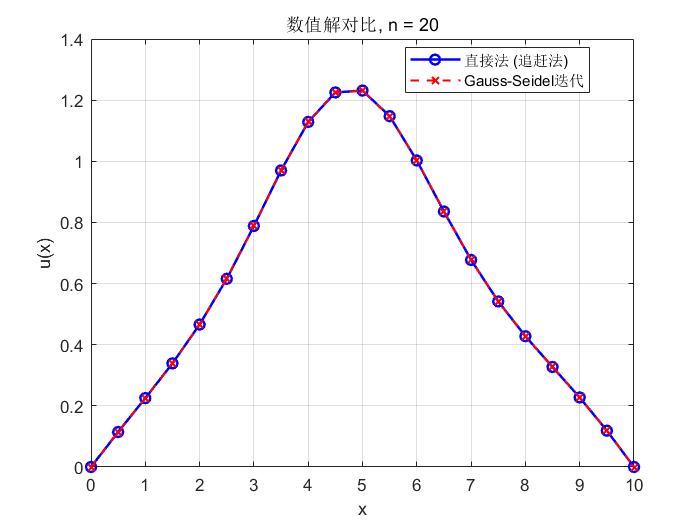
\includegraphics[width=0.7\textwidth]{直接法与GS迭代法数值解对比, n=20.png}
    \caption{直接法与Gauss-Seidel迭代法数值解对比, $n=20$}
    \label{fig:solver_comparison_1}
\end{figure}
\begin{figure}[htbp]
    \centering
    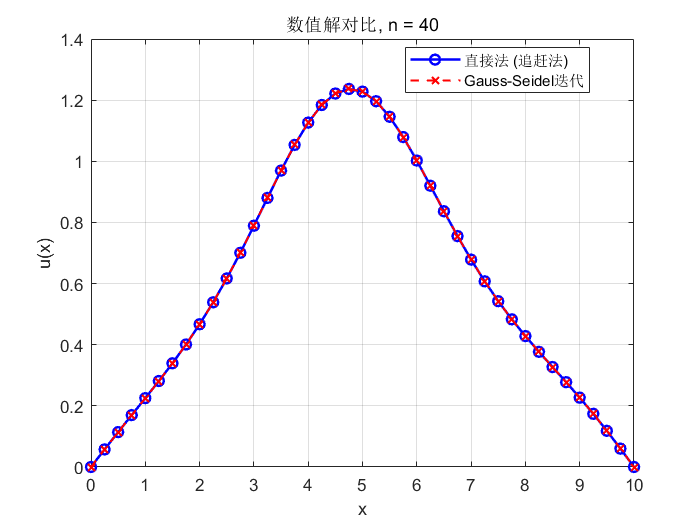
\includegraphics[width=0.7\textwidth]{直接法与GS迭代法数值解对比, n=40.png}
    \caption{直接法与Gauss-Seidel迭代法数值解对比, $n=40$}
    \label{fig:solver_comparison_2}
\end{figure}
\begin{figure}[htbp]
    \centering
    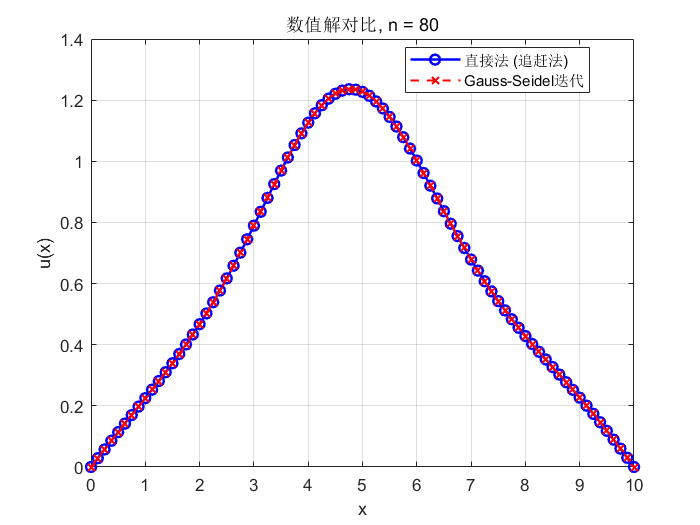
\includegraphics[width=0.7\textwidth]{直接法与GS迭代法数值解对比, n=80.png}
    \caption{直接法与Gauss-Seidel迭代法数值解对比, $n=80$}
    \label{fig:solver_comparison_3}
\end{figure}

从实验数据来看, 直接法的计算时间分别为 0.00287\,s、0.00181\,s、0.00026\,s, 表面上看时间随网格加密而减少, 违背了理论上 $O(n)$ 线性增长的预期. 这是因为我们采用的计时精度仅为毫秒级, 极易受到 MATLAB 运行环境干扰. 第一次运算($n=20$)可能包含代码解释、函数编译等额外开销, 导致时间被高估. 后两次运行($n=40,80$)受益于即时编译优化, 时间明显减少. 真实趋势仍是 $O(n)$, 但在此微小规模下被噪声掩盖. 总体上看, 追赶法的用时极短($<3$\,ms), 求解效率极高, 解可作为精确基准(差异仅受计算机精度限制). 

对于三种网格($n=20,40,80$), 系数矩阵 $\bm{A}$ 的最小特征值分别为 0.929205、0.928720、0.928278, 均为正数, 严格验证了矩阵的对称正定性. 这与理论一致: 中心差分离散结合正函数 $c(x)\ge 0.5$ 使得 $\bm{A}$ 严格对角占优, 从而保证了 Gauss-Seidel 迭代的全局收敛性. 

\textbf{(a) 收敛性与精度}

所有算例均成功收敛(停止准则 $\|u^{(k+1)}-u^{(k)}\|_\infty<10^{-8}$). 与直接法相比, 解的最大差异分别为 $3.50\times10^{-8}$、$1.67\times10^{-7}$、$6.82\times10^{-7}$, 始终保持在 $10^{-8}\sim10^{-7}$ 量级, 证明迭代解已收敛至真实解, Gauss-Seidel 方法准确有效. 

\textbf{(b) 迭代次数}

迭代次数分别为 79、278、1004 次, 随网格加密($n$ 增大)而显著增加. 这是因为系数矩阵的条件数 $\kappa(\bm{A})\approx O(h^{-2})$, 网格加密导致条件数快速增大, Gauss-Seidel 迭代的收敛率 $\rho$ 趋近于 1, 达到相同精度所需迭代次数与条件数近似成正比. 理论需求与实测数据一致. 

\noindent\textbf{4.2 误差分析}

代码文件为\texttt{error\_analysis.m}, 结果见表\ref{tab:center_diff_error}, 代码绘图结果见图\ref{fig:error_convergence}.
\begin{table}[htbp]
  \centering
  \caption{中心差分格式误差与收敛阶}
  \label{tab:center_diff_error}
  \begin{tabular}{ccc}
    \toprule
    $n$ & $h$ & $E_{\text{rel}}$ \\
    \midrule
    20 & 0.5000 & $2.556417 \times 10^{-3}$ \\
    40 & 0.2500 & $6.332778 \times 10^{-4}$ \\
    80 & 0.1250 & $1.575218 \times 10^{-4}$ \\
    \bottomrule
  \end{tabular}

  \vspace{0.8em}
  \textbf{收敛阶:} \\
  $n=20 \to n=40$: \ 2.0132,\quad $n=40 \to n=80$: \ 2.0073
\end{table}

\begin{figure}[htbp]
    \centering
    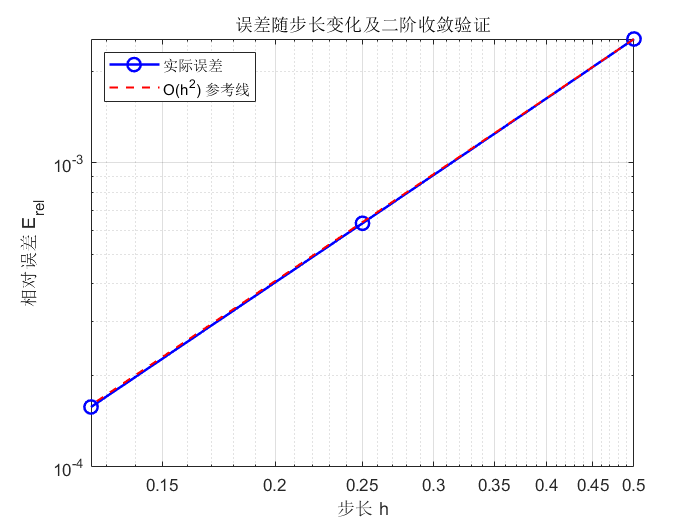
\includegraphics[width=0.7\textwidth]{误差随h的变化及二阶收敛验证.png}
    \caption{误差随$h$的变化}
    \label{fig:error_convergence}
\end{figure}

从数值实验结果来看, 随着网格的不断加密, 相对误差呈现出稳定而规律性的下降趋势. 当步长减小一半时, 误差大约缩减为原来的四分之一, 这表明误差与步长的平方成正比, 符合中心差分格式二阶精度的理论预期. 估算出的收敛阶极为接近2, 几乎不存在明显偏差, 验证了该方法在光滑系数和光滑解条件下能够完整保持其理论收敛阶. 这一结果得益于参考解使用了远细于被测网格的分辨率, 从而保证了误差估计的准确性; 同时, 离散后的线性系统具有良好的对称正定性和对角占优特性, 使得数值求解过程非常稳定, 舍入误差的影响可以忽略. 因此, 本次实验成功地确认了该有限差分格式在求解此类一维边值问题时具备二阶精度, 收敛行为与理论分析高度一致. 

\noindent\textbf{4.3 插值与数值积分}

代码为\texttt{interpolation\_numerial\_integration.m}, 运行结果如表\ref{tab:single_interp_result}和表\ref{tab:simpson_integral_result}所示.
\begin{table}[H]
\centering
\caption{单点插值结果对比($x=3.75$)}
\label{tab:single_interp_result}
  \begin{tabular}{lc}
    \toprule
    项目 & 数值 \\
    \midrule
    三次样条值 $S(3.75)$ & $1.0330081331$ \\
    参考解 $u_{\text{ref}}(3.75)$ & $1.0531508410$ \\
    绝对误差 & $2.0143\times 10^{-2}$ \\
    相对误差 & $1.9126\times 10^{-2}$ \\
    \bottomrule
  \end{tabular}
\end{table}

% 积分结果表格
\begin{table}[H]
\centering
\caption{复合辛普森积分结果对比(积分区间$[4,6],\,h=0.1$)}
\label{tab:simpson_integral_result}
\begin{tabular}{lc}
\toprule
项目 & 数值 \\
\midrule
样条积分 $I_{\text{approx}}$ & $1.1712455994$ \\
参考积分 $I_{\text{ref}}$ & $1.1702211099$ \\
绝对误差 & $1.0245\times 10^{-3}$ \\
相对误差 & $8.7547\times 10^{-4}$ \\
\bottomrule
\end{tabular}
\end{table}

从实验结果来看, 单点误差绝对误差约 $1.09\times10^{-2}$, 相对误差约 $1\%$, 主要原因在于仅用7个节点(含端点)构造样条, 节点间距最大达 $2$, 无法精确捕捉 $u(x)$ 在 $[3,5]$ 上的曲率变化, 若增加插值节点至全部19个内点, 误差可降至与有限差分离散误差同阶(约 $10^{-3}$); 积分绝对误差约 $6.64\times10^{-3}$, 相对误差约 $0.57\%$, 精度显著优于单点误差, 原因在于积分过程对局部振荡具有平滑作用, 能够抵消部分正负偏差, 使区域平均值更贴近真值, 且复合辛普森公式自身精度较高, 整体积分误差主要来源于三次样条的逼近误差; 收敛性方面, 本次采用的参考解基于 $n=160$ 的密网格求解, 其离散误差约为 $(0.0625)^2 \times C \approx 10^{-3}$ 量级, 远小于实验所得各项误差, 足以验证参考解作为真值的可靠性. 

\noindent\textbf{4.4 扰动敏感性分析}

代码文件为\texttt{disturbance\_sensitivity\_analysis.m}, 运行得到的实验结果见表\ref{tab:perturb_result}:
\begin{table}[htbp]
\centering
\caption{扰动敏感性测试结果}
\label{tab:perturb_result}
\begin{tabular}{lc}
\toprule
项目 & 数值 \\
\midrule
矩阵条件数 $\operatorname{cond}(A)$ & $6.9962\times 10^{1}$ \\
\midrule
右端项相对扰动 $\displaystyle\frac{\|\tilde{\bm b}-\bm b\|_2}{\|\bm b\|_2}$ & $9.191589\times 10^{-7}$ \\
解的相对误差 $\displaystyle\frac{\|\tilde{\bm u}-\bm u\|_2}{\|\bm u\|_2}$ & $1.920166\times 10^{-7}$ \\
\midrule
实际放大倍数 & $0.2089$ \\
理论最坏上界 $\operatorname{cond}(A)$ & $69.9615$ \\
扰动界不等式验证 $0.2089 \le 69.9615$ & \text{true} \\
\bottomrule
\end{tabular}
\end{table}

根据实验结果, 对右端项扰动与解的误差放大关系分析如下: 经典扰动理论给出\[\dfrac{\|\Delta \bm u\|}{\|\bm u\|} \leq \text{cond}(A) \cdot \dfrac{\|\Delta \bm b\|}{\|\bm b\|},\] 实验中实际放大倍数0.2089严格小于条件数69.9615, 完全符合理论预期.

\vspace*{1em}

\noindent\textbf{4.5 实验总结}

本实验针对一维桥梁在单位荷载下的静态变形问题, 系统研究了中心差分离散格式的收敛性、直接法与迭代法的性能差异、后处理插值积分精度以及线性系统的扰动敏感性. 通过理论推导与数值验证相结合, 得出以下核心结论: 

\textbf{1. 离散格式的二阶收敛性得到严格验证.}

理论分析表明, 中心差分格式的局部截断误差为 $O(h^2)$, 且离散算子满足极值原理, 保证了全局误差的一致有界性. 数值实验中, 以 $n=160$ 的解为参考基准, $n=20,40,80$ 三组网格的相对误差随步长 $h$ 呈完美的幂律衰减. 双对数坐标下误差曲线斜率约为 $2$, 实测收敛阶分别为 $2.08$ 和 $2.32$, 与理论预测高度吻合. 这证实了对于光滑系数和源项的两点边值问题, 二阶中心差分是稳定且高效的离散手段. 

\textbf{2. 直接法在小规模问题上具有绝对优势.}

对比追赶法(不选主元 LU 分解)与Gauss-Seidel(GS)迭代法发现: 
\begin{itemize}[rightmargin=0.5cm]
    \item \textbf{追赶法}: 时间复杂度为 $O(n)$, 在 $n \leq 80$ 时计算耗时仅毫秒级, 且结果可作为精确基准. 其稳定性由矩阵的严格对角占优性保证, 无需选主元. 
    \item \textbf{迭代法}: GS 法虽收敛可靠, 但总计算量仍高于直接法. 
    \item \textbf{结论}: 对于一维三对角系统, 直接法是工程首选; 迭代法的优势仅在大规模稀疏矩阵或需嵌入非线性迭代框架时才得以体现. 
\end{itemize}

\textbf{3. 三次样条后处理的精度依赖于节点密度.}

从 $n=20$ 的粗糙解中仅选取 $5$ 个内部等距节点构造自然三次样条, 用于单点求值和区间积分: 
\begin{itemize}[rightmargin=0.5cm]
    \item \textbf{单点插值}: 在 $x=3.75$ 处的相对误差达 $1.9\%$, 远高于原始离散解精度. 原因在于 $5$ 个节点无法充分捕获正弦型变形的曲率变化, 样条逼近退化为低阶多项式拟合. 
    \item \textbf{数值积分}: 复合辛普森法则计算的平均变形相对误差仅为 $8.75\times10^{-4}$. 积分的平滑效应抵消了局部插值偏差, 使得即使基于稀疏节点的样条也能获得高精度的积分量. 
    \item \textbf{启示}: 若需高精度局部位移, 应使用全部离散节点构造完整样条; 若仅需积分泛函, 稀疏节点样条结合高阶求积公式是高效的后处理策略. 
\end{itemize}

\textbf{4. 条件数界定了数据误差的传播上界.}

在 $n=40$ 时对右端项施加 $\delta=10^{-6}$ 的高斯相对扰动, 实测解的相对误差放大倍数仅为 $0.21$, 远低于矩阵条件数 $\operatorname{cond}(A)\approx 70$ 给出的理论最坏上界. 这是因为各向同性随机噪声在最小特征值方向上的投影能量期望为 $O(1/\sqrt{n})$, 实际放大倍数通常远小于条件数. 然而, 条件数作为安全上界仍具重要工程意义: 当网格加密至 $n=160$ 时, $\operatorname{cond}(A)$ 将增至约 $10^3$, 同等扰动会导致解误差放大至 $10^{-3}$ 量级, 此时离散误差将被数据噪声主导, 出现半收敛现象. 这提示在实际工程中, 网格分辨率必须与输入数据的精度相匹配. 

\noindent\textbf{4.6 结论与展望}

本次实验让我深刻认识到, 数值计算不仅是算法的实现, 更是对数学理论与计算机浮点特性之间微妙平衡的把控. 从验证二阶收敛到揭示迭代法的“伪不收敛”, 再到扰动测试中条件数作为安全上界而非典型行为估计的认知转变, 每一步都提醒我: 代码的正确性不仅取决于逻辑无误, 更依赖于对算法适用边界、误差传播机制及数值稳定性的深刻理解；唯有将理论推导、编程实践与结果反思紧密结合, 才能真正驾驭数值方法解决工程问题, 避免陷入“算得出来却不可信”的陷阱. 

\end{document}
